

\section{Komplexe Zahlen}

\begin{lemma}{Fundamentalsatz der Algebra}\\
Eine algebraische Gleichung n-ten Grades mit komplexen Koeffizienten:
$$a_nz^n + a_{n-1}z^{n-1} + \cdots + a_1z + a_0 = 0$$
besitzt in $\mathbb{C}$ genau n Lösungen (mit Vielfachheiten gezählt).
\end{lemma}

\begin{concept}{Komplexe Zahlen}\\
Die Menge der komplexen Zahlen $\mathbb{C}$ erweitert die reellen Zahlen $\mathbb{R}$ durch Einführung der imaginären Einheit $i$ mit der Eigenschaft:
$$i^2 = -1$$

Eine komplexe Zahl $z$ ist ein geordnetes Paar $(x,y)$ mit $x,y \in \mathbb{R}$:
$$z = x + iy$$

Die Menge aller komplexen Zahlen ist definiert als:
$$\mathbb{C} = \{z \mid z = x + iy \text{ mit } x,y \in \mathbb{R}\}$$
\end{concept}

\begin{definition}{Bestandteile komplexer Zahlen}\\
\begin{minipage}[t]{0.6\textwidth}
    \vspace{-7mm}
    \textbf{Realteil:} $\operatorname{Re}(z) = x$\\
    \textbf{Imaginärteil:} $\operatorname{Im}(z) = y$\\
    \textbf{Betrag:} $|z| = \sqrt{x^2 + y^2} = \sqrt{z \cdot z^*}$\\
    \textbf{Konjugation:} $\overline{z} = x - iy$
\end{minipage}
\begin{minipage}{0.35\textwidth}
    \vspace{-3mm}
    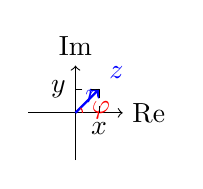
\begin{tikzpicture}[scale=0.3]
        % Coordinate axes
        \draw[->] (-2,0) -- (2,0) node[right] {Re};
        \draw[->] (0,-2) -- (0,2) node[above] {Im};
        
        % Example point and vector
        \draw[thick,blue,->] (0,0) -- (1,1) node[above right] {$z$};
        
        % Angle and labels
        \draw[red] (0.3,0) arc (0:45:0.3) node[midway,right] {$\varphi$};
        
        % Components
        \draw[dashed] (1,1) -- (1,0) node[below] {$x$};
        \draw[dashed] (1,1) -- (0,1) node[left] {$y$};
        
        % Radius
        \node[blue] at (0.7,0.7) {$r$};
    \end{tikzpicture}
\end{minipage}
\end{definition}


\begin{concept}{Darstellungsformen}
\begin{itemize}
    \item Normalform: $z = x + iy$
    \item Trigonometrische Form: $z = r(\cos\varphi + i\sin\varphi)$
    \item Exponentialform: $z = re^{i\varphi}$
\end{itemize}
\end{concept}

\begin{KR}{Umrechnung zwischen Darstellungsformen komplexer Zahlen}
\paragraph{Von Normalform in trigonometrische Form/Exponentialform}
\begin{enumerate}
   \item Berechne Betrag $r = \sqrt{x^2 + y^2}$
   \item Berechne Winkel mit einer der Formeln: 
   \begin{itemize}
       \item $\varphi = \arctan(\frac{y}{x})$ falls $x > 0$
       \item $\varphi = \arctan(\frac{y}{x}) + \pi$ falls $x < 0$
       \item $\varphi = \frac{\pi}{2}$ falls $x = 0, y > 0$
       \item $\varphi = -\frac{\pi}{2}$ falls $x = 0, y < 0$
       \item $\varphi$ unbestimmt falls $x = y = 0$
   \end{itemize}
   \item Trigonometrische Form: $z = r(\cos\varphi + i\sin\varphi)$
   \item Exponentialform: $z = re^{i\varphi}$
\end{enumerate}

\paragraph{Von trigonometrischer Form in Normalform}
\begin{enumerate}
   \item Realteil: $x = r\cos\varphi$
   \item Imaginärteil: $y = r\sin\varphi$
   \item Normalform: $z = x + iy$
\end{enumerate}

\paragraph{Von Exponentialform in Normalform/trigonometrische Form}
\begin{enumerate}
   \item Trigonometrische Form durch Euler-Formel:\\
   $re^{i\varphi} = r(\cos\varphi + i\sin\varphi)$
   \item Dann wie oben in Normalform umrechnen
\end{enumerate}

\paragraph{Wichtige Hinweise:}
\begin{itemize}
   \item Achten Sie auf das korrekte Quadranten beim Winkel
   \item Winkelfunktionen im Bogenmaß verwenden
   \item Bei Umrechnung in Normalform Euler-Formel nutzen
   \item Vorzeichen bei Exponentialform beachten
\end{itemize}
\end{KR}

\begin{KR}{Komplexe Zahlen umrechnen}
\begin{enumerate}
    \item Normalform $\leftrightarrow$ Polarform:
    \begin{itemize}
        \item Betrag: $r = \sqrt{x^2 + y^2}$
        \item Winkel: $\varphi = \arctan(\frac{y}{x})$ (Quadrant beachten!)
        \item Normalform: $z = x + iy$
        \item Polarform: $z = r(\cos\varphi + i\sin\varphi) = re^{i\varphi}$
    \end{itemize}
    
    \item Rechenoperationen:
    \begin{itemize}
        \item Addition: $(x_1 + iy_1) + (x_2 + iy_2) = (x_1+x_2) + i(y_1+y_2)$
        \item Multiplikation: $r_1r_2e^{i(\varphi_1 + \varphi_2)}$
        \item Division: $\frac{r_1}{r_2}e^{i(\varphi_1 - \varphi_2)}$
        \item n-te Potenz: $r^ne^{in\varphi}$
    \end{itemize}
\end{enumerate}
\end{KR}

\begin{example2}{Komplexe Operationen}
Gegeben $z_1 = 1+i$ und $z_2 = 2-i$:

\paragraph{Umrechnung in Polarform:}
\begin{itemize}
    \item $z_1: r_1 = \sqrt{2}$, $\varphi_1 = \frac{\pi}{4}$
    \item $z_2: r_2 = \sqrt{5}$, $\varphi_2 = -\arctan(\frac{1}{2})$
\end{itemize}

\paragraph{Berechnungen:}
\begin{itemize}
    \item $z_1 \cdot z_2 = (2-i)(1+i) = (2+1) + i(2-1) = 3+i$
    \item $z_1^3 = (\sqrt{2})^3(\cos(\frac{3\pi}{4}) + i\sin(\frac{3\pi}{4}))$
\end{itemize}
\end{example2}

\begin{theorem}{Rechenoperationen mit komplexen Zahlen}\\
Für $z_1 = x_1 + iy_1$ und $z_2 = x_2 + iy_2$ gilt:
\vspace{1mm}\\
\begin{minipage}[t]{0.45\textwidth}
    \textbf{Addition:}\\
    $z_1 + z_2 = (x_1 + x_2) + i(y_1 + y_2)$
\end{minipage}
\hspace{3mm}
\begin{minipage}[t]{0.45\textwidth}
    \textbf{Subtraktion:}\\
    $z_1 - z_2 = (x_1 - x_2) + i(y_1 - y_2)$
\end{minipage}

\begin{minipage}{0.28\textwidth}
    \textbf{Multiplikation:}
\end{minipage}
\begin{minipage}{0.68\textwidth}
    \begin{align*}
        z_1 \cdot z_2 &= (x_1x_2 - y_1y_2) + i(x_1y_2 + x_2y_1)\\
        &= r_1r_2e^{i(\varphi_1 + \varphi_2)} \text{ (in Exponentialform)}
    \end{align*}
\end{minipage}



\textbf{Division:}
\begin{align*}
    \frac{z_1}{z_2} &= \frac{z_1 \cdot z_2^*}{z_2 \cdot z_2^*} = \frac{(x_1x_2 + y_1y_2) + i(y_1x_2 - x_1y_2)}{x_2^2 + y_2^2}\\
    &= \frac{r_1}{r_2}e^{i(\varphi_1 - \varphi_2)} \text{ (in Exponentialform)}
\end{align*}
\end{theorem}

\begin{theorem}{Potenzen und Wurzeln}\\
Für eine komplexe Zahl in Exponentialform $z = re^{i\varphi}$ gilt:
\begin{itemize}
    \item n-te Potenz: $z^n = r^ne^{in\varphi} = r^n(\cos(n\varphi) + i\sin(n\varphi))$
    \item n-te Wurzel: $z_k = \sqrt[n]{r}e^{i\frac{\varphi + 2\pi k}{n}}$, $k = 0,1,\ldots,n-1$
\end{itemize}
\end{theorem}


\section{Eigenwerte und Eigenvektoren}

\begin{definition}{Eigenwerte und Eigenvektoren}\\
Für eine Matrix $A \in \mathbb{R}^{n\times n}$ heißt $\lambda \in \mathbb{C}$ Eigenwert von $A$, wenn es einen Vektor $x \in \mathbb{C}^n \backslash \{0\}$ gibt mit:
\vspace{-2mm}\\
$$Ax = \lambda x$$
Der Vektor $x$ heißt dann Eigenvektor zum Eigenwert $\lambda$.
\end{definition}

\begin{concept}{Bestimmung von Eigenwerten}\\
Ein Skalar $\lambda$ ist genau dann Eigenwert von $A$, wenn gilt:
\vspace{-2mm}\\
$$\det(A - \lambda I_n) = 0$$
Diese Gleichung heißt charakteristische Gleichung. Das zugehörige Polynom
\vspace{-2mm}
$$p(\lambda) = \det(A - \lambda I_n)$$
ist das charakteristische Polynom von $A$.
\end{concept}

\begin{theorem}{Eigenschaften von Eigenwerten}
Für eine Matrix $A \in \mathbb{R}^{n\times n}$ gilt:
$$\det(A) = \prod_{i=1}^n \lambda_i \text{ (Produkt der Eigenwerte)}$$
$$\operatorname{tr}(A) = \sum_{i=1}^n \lambda_i \text{ (Summe der Eigenwerte)}$$
\begin{itemize}
    \item Bei Dreiecksmatrix sind die Diagonalelemente die Eigenwerte
    \item Ist $\lambda$ Eigenwert von $A$, so ist $\frac{1}{\lambda}$ Eigenwert von $A^{-1}$
\end{itemize}
\end{theorem}

\begin{concept}{Vielfachheiten}
Für einen Eigenwert $\lambda$ unterscheidet man:
\begin{itemize}
    \item Algebraische Vielfachheit: \\Vielfachheit als Nullstelle des charakteristischen Polynoms
    \item Geometrische Vielfachheit: \\Dimension des Eigenraums $= n - \operatorname{rg}(A-\lambda I_n)$
\end{itemize}
Die geometrische Vielfachheit ist stets kleiner oder gleich der algebraischen Vielfachheit.
\end{concept}

\begin{KR}{Bestimmung von Eigenwerten und Eigenvektoren}
\paragraph{Vorbereitung}
\begin{itemize}
    \item Matrix $A \in \mathbb{R}^{n \times n}$ aufschreiben
    \item Charakteristische Matrix $(A - \lambda I)$ aufstellen
\end{itemize}

\paragraph{Eigenwerte bestimmen}
\begin{enumerate}
    \item Charakteristisches Polynom aufstellen:
    \begin{itemize}
        \item Bei $2 \times 2$ Matrizen direkt: $\det(A - \lambda I)$
        \item Bei $3 \times 3$ Matrizen: Entwicklung nach einer Zeile/Spalte
        \item Bei größeren Matrizen: Spezielle Eigenschaften nutzen
              (z.B. Dreiecksform, Symmetrie)
    \end{itemize}
    
    \item Polynom vereinfachen und auf Nullform bringen:
    \begin{itemize}
        \item Ausmultiplizieren
        \item Zusammenfassen nach Potenzen von $\lambda$
        \item Form: $p(\lambda) = (-1)^n\lambda^n + a_{n-1}\lambda^{n-1} + \cdots + a_1\lambda + a_0$
    \end{itemize}

    \item Nullstellen bestimmen:
    \begin{itemize}
        \item Bei quadratischer Gleichung: Mitternachtsformel
        \item Bei Grad 3: Substitution oder Cardanische Formeln
        \item Bei höherem Grad: Numerische Verfahren
    \end{itemize}
\end{enumerate}

\paragraph{Eigenvektoren bestimmen}
\begin{enumerate}
    \item Für jeden Eigenwert $\lambda_i$:
    \begin{itemize}
        \item Matrix $(A - \lambda_i I)$ aufstellen
        \item Homogenes LGS $(A - \lambda_i I)x = 0$ lösen
        \item Lösungsvektor normieren falls gewünscht
    \end{itemize}

    \item Bei mehrfachen Eigenwerten:
    \begin{itemize}
        \item Basis des Eigenraums bestimmen
        \item Linear unabhängige Eigenvektoren finden
    \end{itemize}
\end{enumerate}

\paragraph{Kontrolle}
\begin{itemize}
    \item Für jeden Eigenvektor $x_i$ prüfen: $Ax_i = \lambda_i x_i$
    \item Bei $2 \times 2$ Matrix: $\lambda_1 + \lambda_2 = \operatorname{tr}(A)$ und $\lambda_1 \cdot \lambda_2 = \det(A)$
    \item Bei $3 \times 3$ Matrix zusätzlich: $\sum \lambda_i = \operatorname{tr}(A)$ und $\prod \lambda_i = \det(A)$
    \item Bei reellen Matrizen: Komplexe Eigenwerte treten in konjugierten Paaren auf
\end{itemize}

\paragraph{Spezialfälle beachten}
\begin{itemize}
    \item Bei Dreiecksmatrizen: Eigenwerte sind die Diagonalelemente
    \item Bei symmetrischen Matrizen: Alle Eigenwerte sind reell
    \item Bei orthogonalen Matrizen: $|\lambda_i| = 1$ für alle Eigenwerte
    \item Bei nilpotenten Matrizen: Alle Eigenwerte sind 0
\end{itemize}
\end{KR}

\begin{example2}{Eigenwertberechnung}
Gegeben ist die Matrix
$A = \begin{psmallmatrix} 
2 & 1 & 0 \\
1 & 2 & 1 \\
0 & 1 & 2
\end{psmallmatrix}$

1. Charakteristisches Polynom aufstellen:
   $$\det(A - \lambda I) = \begin{vsmallmatrix} 
   2-\lambda & 1 & 0 \\
   1 & 2-\lambda & 1 \\
   0 & 1 & 2-\lambda
   \end{vsmallmatrix}$$
   
2. Entwicklung nach 1. Zeile:
   $$p(\lambda) = (2-\lambda)\begin{vsmallmatrix}
   2-\lambda & 1 \\
   1 & 2-\lambda
   \end{vsmallmatrix} - 1\begin{vsmallmatrix}
   1 & 1 \\
   1 & 2-\lambda
   \end{vsmallmatrix}$$
   
3. Ausrechnen:
   $$p(\lambda) = (2-\lambda)((2-\lambda)^2 - 1) - ((2-\lambda) - 1)
   = -\lambda^3 + 6\lambda^2 - 11\lambda + 6$$
   
4. Nullstellen bestimmen:
   $\lambda_1 = 1, \lambda_2 = 2, \lambda_3 = 3$
\vspace{1mm}\\
5. Eigenvektoren bestimmen für $\lambda_1 = 1$:
   $$(A - I)x = 0 \text{ führt zu } x_1 = \begin{psmallmatrix} 1 \\ -2 \\ 1 \end{psmallmatrix}$$
\end{example2}

\begin{KR}{Eigenwerte bestimmen}
\begin{enumerate}
    \item Charakteristisches Polynom aufstellen:
    \begin{itemize}
        \item $p(\lambda) = \det(A-\lambda I)$ berechnen
        \item Auf Standardform bringen
    \end{itemize}
    
    \item Nullstellen bestimmen:
    \begin{itemize}
        \item Quadratische Formel für $n=2$
        \item Cardano-Formel für $n=3$
        \item Numerische Verfahren für $n>3$
    \end{itemize}
    
    \item Vielfachheiten bestimmen:
    \begin{itemize}
        \item Algebraische Vielfachheit: Nullstellenordnung
        \item Geometrische Vielfachheit: $n-\operatorname{rang}(A-\lambda I)$
    \end{itemize}
\end{enumerate}
\end{KR}

\begin{example2}{Charakteristisches Polynom}
Bestimmen Sie die Eigenwerte von:
$$A = \begin{pmatrix}
2 & -1 & 0 \\
-1 & 2 & -1 \\
0 & -1 & 2
\end{pmatrix}$$

\paragraph{Lösung:}
\begin{enumerate}
    \item $p(\lambda) = \det(A-\lambda I)$:
    $$\begin{vmatrix}
    2-\lambda & -1 & 0 \\
    -1 & 2-\lambda & -1 \\
    0 & -1 & 2-\lambda
    \end{vmatrix}$$
    
    \item Determinante entwickeln:
    $$p(\lambda) = (2-\lambda)^3 - 2(2-\lambda) = -\lambda^3 + 6\lambda^2 - 11\lambda + 6$$
    
    \item Nullstellen:
    $$\lambda_1 = 1, \lambda_2 = 2, \lambda_3 = 3$$
\end{enumerate}
\end{example2}

\begin{KR}{Eigenvektoren bestimmen}
\begin{enumerate}
    \item Für jeden Eigenwert $\lambda$:
    \begin{itemize}
        \item $(A-\lambda I)x = 0$ aufstellen
        \item Homogenes LGS lösen
        \item Lösungsvektor normieren
    \end{itemize}
    
    \item Bei mehrfachen Eigenwerten:
    \begin{itemize}
        \item Geometrische Vielfachheit bestimmen
        \item Basis des Eigenraums finden
    \end{itemize}
    
    \item Kontrolle:
    \begin{itemize}
        \item $Ax = \lambda x$ überprüfen
        \item Orthogonalität bei symmetrischen Matrizen
        \item Linear unabhängig?
    \end{itemize}
\end{enumerate}
\end{KR}

\begin{example2}{Eigenvektoren}
Bestimmen Sie die Eigenvektoren zum Eigenwert $\lambda=2$ der Matrix:
$$A = \begin{pmatrix}
2 & 1 & 0 \\
0 & 2 & 0 \\
0 & -1 & 2
\end{pmatrix}$$

\paragraph{Lösung:}
\begin{enumerate}
    \item $(A-2I)x = 0$:
    $$\begin{pmatrix}
    0 & 1 & 0 \\
    0 & 0 & 0 \\
    0 & -1 & 0
    \end{pmatrix} \begin{pmatrix}
    x_1 \\ x_2 \\ x_3
    \end{pmatrix} = \begin{pmatrix}
    0 \\ 0 \\ 0
    \end{pmatrix}$$
    
    \item Homogenes System lösen:
    \begin{itemize}
        \item $x_2 = 0$ (aus 1. Zeile)
        \item $x_1, x_3$ frei wählbar
    \end{itemize}
    
    \item Basis des Eigenraums:
    $$v_1 = \begin{pmatrix} 1 \\ 0 \\ 0 \end{pmatrix}, 
    v_2 = \begin{pmatrix} 0 \\ 0 \\ 1 \end{pmatrix}$$
\end{enumerate}
\end{example2}

\subsubsection{Numerische Berechnung von Eigenwerten}

\begin{concept}{Ähnliche Matrizen}\\
Zwei Matrizen $A,B \in \mathbb{R}^{n\times n}$ heißen ähnlich, wenn es eine reguläre Matrix $T$ gibt mit:
$$B = T^{-1}AT$$

Eine Matrix $A$ heißt diagonalisierbar, wenn sie ähnlich zu einer Diagonalmatrix $D$ ist:
$$D = T^{-1}AT$$
\end{concept}

\begin{theorem}{Eigenschaften ähnlicher Matrizen}\\
Für ähnliche Matrizen $A$ und $B = T^{-1}AT$ gilt:
\begin{enumerate}
    \item $A$ und $B$ haben dieselben Eigenwerte mit gleichen algebraischen Vielfachheiten
    \item Ist $x$ Eigenvektor von $B$ zum Eigenwert $\lambda$, so ist $Tx$ Eigenvektor von $A$ zum Eigenwert $\lambda$
    \item Bei Diagonalisierbarkeit:
    \begin{itemize}
        \item Die Diagonalelemente von $D$ sind die Eigenwerte von $A$
        \item Die Spalten von $T$ sind die Eigenvektoren von $A$
    \end{itemize}
\end{enumerate}
\end{theorem}

\begin{definition}{Spektralradius}
Der Spektralradius einer Matrix $A$ ist definiert als:
$$\rho(A) = \max\{|\lambda| \mid \lambda \text{ ist Eigenwert von } A\}$$
Er gibt den Betrag des betragsmäßig größten Eigenwerts an.
\end{definition}

\subsubsection{Von-Mises-Iteration}

\begin{concept}{Von-Mises-Iteration (Vektoriteration)}\\
Für eine diagonalisierbare Matrix $A$ mit Eigenwerten $|\lambda_1| > |\lambda_2| \geq \cdots \geq |\lambda_n|$ konvergiert die Folge:
$$v^{(k+1)} = \frac{Av^{(k)}}{\|Av^{(k)}\|_2}, \quad
\lambda^{(k+1)} = \frac{(v^{(k)})^TAv^{(k)}}{(v^{(k)})^Tv^{(k)}}$$
gegen einen Eigenvektor $v$ zum betragsmäßig größten Eigenwert $\lambda_1$.
\end{concept}

\begin{KR}{Von-Mises-Iteration / Vektoriteration}
\paragraph{Algorithmus}
\begin{enumerate}
    \item Startvektor $v^{(0)}$ wählen:
    \begin{itemize}
        \item Zufälligen Vektor oder $(1,\ldots,1)^T$ wählen
        \item Auf Länge 1 normieren: $\|v^{(0)}\|_2 = 1$
    \end{itemize}

    \item Für $k = 0,1,2,\ldots$ bis zur Konvergenz:
    \begin{itemize}
        \item Iterationsvektor berechnen: $w^{(k)} = Av^{(k)}$
        \item Normieren: $v^{(k+1)} = \frac{w^{(k)}}{\|w^{(k)}\|_2}$
        \item Eigenwertapproximation (Rayleigh-Quotient):
              $$\lambda^{(k+1)} = \frac{(v^{(k)})^TAv^{(k)}}{(v^{(k)})^Tv^{(k)}}$$
    \end{itemize}

    \item Abbruchkriterien prüfen:
    \begin{itemize}
        \item Änderung des Eigenvektors: $\|v^{(k+1)} - v^{(k)}\| < \varepsilon$
        \item Änderung des Eigenwertes: $|\lambda^{(k+1)} - \lambda^{(k)}| < \varepsilon$
        \item Maximale Iterationszahl erreicht
    \end{itemize}
\end{enumerate}

\paragraph{Verifikation}
\begin{itemize}
    \item Prüfen ob $Av^{(k)} \approx \lambda^{(k)}v^{(k)}$
    \item Residuum berechnen: $\|Av^{(k)} - \lambda^{(k)}v^{(k)}\|$
    \item Orthogonalität zu anderen Eigenvektoren prüfen
\end{itemize}
\end{KR}

\begin{example2}{Von-Mises-Iteration}
Gegeben sei die Matrix
$A = \begin{psmallmatrix} 
4 & -1 & 1 \\
-1 & 3 & -2 \\
1 & -2 & 3
\end{psmallmatrix}$

Mit Startvektor $v^{(0)} = \frac{1}{\sqrt{3}}(1,1,1)^T$:

\begin{enumerate}
    \item Erste Iteration:
    \begin{itemize}
        \item $w^{(0)} = Av^{(0)} = \frac{1}{\sqrt{3}}(4,0,2)^T$
        \item $v^{(1)} = \frac{w^{(0)}}{\|w^{(0)}\|} = \frac{1}{\sqrt{20}}(4,0,2)^T$
        \item $\lambda^{(1)} = (v^{(0)})^TAv^{(0)} = 3.33$
    \end{itemize}

    \item Zweite Iteration:
    \begin{itemize}
        \item $w^{(1)} = Av^{(1)} = \frac{1}{\sqrt{20}}(18,-2,8)^T$
        \item $v^{(2)} = \frac{w^{(1)}}{\|w^{(1)}\|} = \frac{1}{\sqrt{388}}(18,-2,8)^T$
        \item $\lambda^{(2)} = 5.12$
    \end{itemize}

Konvergenz gegen $\lambda_1 \approx 5.17$ und $v = (0.89, -0.10, 0.39)^T$
\end{enumerate}
\end{example2}

\begin{KR}{Vektoriteration durchführen}
\begin{enumerate}
    \item Voraussetzungen prüfen:
    \begin{itemize}
        \item Matrix diagonalisierbar
        \item $|\lambda_1| > |\lambda_2|$
    \end{itemize}
    
    \item Iteration:
    \begin{itemize}
        \item $w^{(k)} = Av^{(k)}$
        \item $v^{(k+1)} = \frac{w^{(k)}}{\|w^{(k)}\|}$
        \item $\lambda^{(k+1)} = \frac{(v^{(k)})^TAv^{(k)}}{(v^{(k)})^Tv^{(k)}}$
    \end{itemize}
    
    \item Konvergenz:
    \begin{itemize}
        \item $v^{(k)} \to$ Eigenvektor zu $|\lambda_1|$
        \item $\lambda^{(k)} \to |\lambda_1|$
    \end{itemize}
\end{enumerate}
\end{KR}

\begin{example2}{Von-Mises-Iteration}
Bestimmen Sie den betragsmäßig größten Eigenwert von:
$$A = \begin{pmatrix}
3 & 1 \\
1 & 3
\end{pmatrix}$$

\paragraph{Lösung:}
\begin{enumerate}
    \item Start mit $v^{(0)} = \frac{1}{\sqrt{2}}\begin{pmatrix} 1 \\ 1 \end{pmatrix}$
    
    \item Erste Iteration:
    \begin{itemize}
        \item $w^{(0)} = \begin{pmatrix} 4 \\ 4 \end{pmatrix}$
        \item $v^{(1)} = \frac{1}{\sqrt{2}}\begin{pmatrix} 1 \\ 1 \end{pmatrix}$
        \item $\lambda^{(1)} = 4$
    \end{itemize}
    
    \item Ergebnis:
    \begin{itemize}
        \item Eigenvektor bereits gefunden
        \item Eigenwert $\lambda = 4$ ist korrekt
    \end{itemize}
\end{enumerate}
\end{example2}

\subsubsection{QR-Verfahren}

\begin{concept}{QR-Verfahren}\\
Das QR-Verfahren transformiert die Matrix $A$ iterativ in eine obere Dreiecksmatrix, deren Diagonalelemente die Eigenwerte sind:
\begin{enumerate}
    \item Initialisierung: $A_0 := A$, $P_0 := I_n$
    \item Für $i = 0,1,2,\ldots$:
    \begin{itemize}
        \item QR-Zerlegung: $A_i = Q_iR_i$
        \item Neue Matrix: $A_{i+1} = R_iQ_i$
        \item Update: $P_{i+1} = P_iQ_i$
    \end{itemize}
\end{enumerate}
\end{concept}

\begin{KR}{QR-Verfahren}
\paragraph{Voraussetzungen}
\begin{itemize}
    \item Matrix $A \in \mathbb{R}^{n \times n}$
    \item Eigenwerte sollten verschiedene Beträge haben für gute Konvergenz
\end{itemize}

\paragraph{Algorithmus}
\begin{enumerate}
    \item Initialisierung:
    \begin{itemize}
        \item $A_0 := A$
        \item $Q_0 := I_n$
    \end{itemize}

    \item Für $k = 0,1,2,\ldots$ bis zur Konvergenz:
    \begin{itemize}
        \item QR-Zerlegung von $A_k$ berechnen: $A_k = Q_kR_k$
        \item Neue Matrix berechnen: $A_{k+1} = R_kQ_k$
        \item Transformationsmatrix aktualisieren: $P_{k+1} = P_kQ_k$
    \end{itemize}

    \item Abbruchkriterien prüfen:
    \begin{itemize}
        \item Subdiagonalelemente nahe Null: $|a_{i+1,i}| < \varepsilon$
        \item Änderung der Diagonalelemente klein
        \item Maximale Iterationszahl erreicht
    \end{itemize}
\end{enumerate}

\paragraph{Auswertung}
\begin{itemize}
    \item Eigenwerte: Diagonalelemente von $A_k$
    \item Eigenvektoren: Spalten der Matrix $P_k$
    \item Bei $2\times2$-Blöcken: Komplexe Eigenwertpaare
\end{itemize}
\end{KR}

\begin{example2}{QR-Verfahren}
Gegeben sei die Matrix
$A = \begin{psmallmatrix} 
1 & 2 & 0 \\
2 & 1 & 1 \\
0 & 1 & 1
\end{psmallmatrix}$

\begin{enumerate}
    \item Erste Iteration:
    \begin{itemize}
        \item QR-Zerlegung:
        $Q_1 = \begin{psmallmatrix} 
        0.45 & 0.89 & 0 \\
        0.89 & -0.45 & 0 \\
        0 & 0 & 1
        \end{psmallmatrix}$,
        $R_1 = \begin{psmallmatrix}
        2.24 & 2.24 & 0.45 \\
        0 & -1 & 0.89 \\
        0 & 0 & 1
        \end{psmallmatrix}$
        \item $A_1 = R_1Q_1 = \begin{psmallmatrix}
        2.24 & 0.45 & 0.45 \\
        0.45 & 0.38 & 0.89 \\
        0.45 & 0.89 & 1
        \end{psmallmatrix}$
    \end{itemize}

    \item Nach Konvergenz:
    $A_k \approx \begin{psmallmatrix}
    3 & * & * \\
    0 & 0 & * \\
    0 & 0 & 0
    \end{psmallmatrix}$

    Eigenwerte sind also $\lambda_1 = 3, \lambda_2 = 0, \lambda_3 = 0$
\end{enumerate}
\end{example2}

\begin{KR}{QR-Algorithmus anwenden}
\begin{enumerate}
    \item Initialisierung:
    \begin{itemize}
        \item $A_0 := A$
        \item $Q_0 := I_n$
    \end{itemize}
    
    \item Iteration:
    \begin{itemize}
        \item QR-Zerlegung: $A_k = Q_kR_k$
        \item Neue Matrix: $A_{k+1} = R_kQ_k$
        \item Update: $P_{k+1} = P_kQ_k$
    \end{itemize}
    
    \item Abbruch wenn:
    \begin{itemize}
        \item Subdiagonalelemente klein
        \item Diagonalelemente konvergieren
        \item Maximale Iterationen erreicht
    \end{itemize}
\end{enumerate}
\end{KR}

\begin{example2}{QR-Iteration}
Führen Sie eine QR-Iteration durch für:
$$A = \begin{pmatrix}
1 & 1 \\
1 & 0
\end{pmatrix}$$

\paragraph{Lösung:}
\begin{enumerate}
    \item QR-Zerlegung von $A$:
    $$Q_1 = \frac{1}{\sqrt{2}}\begin{pmatrix}
    1 & -1 \\
    1 & 1
    \end{pmatrix}, 
    R_1 = \frac{1}{\sqrt{2}}\begin{pmatrix}
    \sqrt{2} & 1 \\
    0 & -1
    \end{pmatrix}$$
    
    \item Neue Matrix:
    $$A_1 = R_1Q_1 = \begin{pmatrix}
    1.5 & 0.5 \\
    0.5 & -0.5
    \end{pmatrix}$$
    
    \item Konvergenz nach mehreren Iterationen gegen:
    $$A_\infty \approx \begin{pmatrix}
    \phi & 0 \\
    0 & -\phi^{-1}
    \end{pmatrix}$$
    mit $\phi = \frac{1+\sqrt{5}}{2}$
\end{enumerate}
\end{example2}





\begin{KR}{Numerische Aspekte}
\begin{enumerate}
    \item Wahl des Startpunkts:
    \begin{itemize}
        \item Von-Mises: zufälliger normierter Vektor
        \item Inverse Iteration: Näherung für $\mu$ wichtig
        \item QR: Matrix vorher auf Hessenberg-Form
    \end{itemize}
    
    \item Konvergenzprüfung:
    \begin{itemize}
        \item Residuum $\|Ax^{(k)} - \lambda^{(k)}x^{(k)}\|$
        \item Änderung in aufeinanderfolgenden Iterationen
        \item Subdiagonalelemente bei QR
    \end{itemize}
    
    \item Spezialfälle:
    \begin{itemize}
        \item Mehrfache Eigenwerte
        \item Komplexe Eigenwerte/vektoren
        \item Schlecht konditionierte Matrizen
    \end{itemize}
\end{enumerate}
\end{KR}


\subsection{Eigenwerte und Eigenvektoren}

\begin{definition}{Eigenwerte und Eigenvektoren}
Für eine Matrix $A \in \mathbb{R}^{n \times n}$ ist $\lambda \in \mathbb{C}$ ein Eigenwert und $x \in \mathbb{C}^n \setminus \{0\}$ ein zugehöriger Eigenvektor, wenn gilt:
$$Ax = \lambda x$$
\end{definition}

\begin{concept}{Spektralradius}
Der Spektralradius $\rho(A)$ einer Matrix $A$ ist der betragsmäßig größte Eigenwert:
$$\rho(A) = \max\{|\lambda| : \lambda \text{ ist Eigenwert von } A\}$$
Der Spektralradius spielt eine wichtige Rolle bei der Konvergenz iterativer Verfahren.
\end{concept}

\begin{KR}{Bestimmung von Eigenwerten und Eigenvektoren}
\begin{enumerate}
    \item Eigenwerte bestimmen:
    \begin{itemize}
        \item Charakteristisches Polynom aufstellen: $p(\lambda) = \det(A-\lambda I)$
        \item Nullstellen von $p(\lambda)$ finden
    \end{itemize}
    
    \item Für jeden Eigenwert $\lambda$:
    \begin{itemize}
        \item Löse $(A-\lambda I)x = 0$ 
        \item Bestimme Basisvektoren des Eigenraums
        \item Normiere die Eigenvektoren falls gewünscht
    \end{itemize}
    
    \item Bei QR-Verfahren:
    \begin{itemize}
        \item QR-Zerlegung iterativ durchführen
        \item Diagonalelemente konvergieren gegen Eigenwerte
        \item Produkt der Q-Matrizen ergibt Eigenvektoren
    \end{itemize}
\end{enumerate}
\end{KR}

\begin{example2}{Eigenwerte und Eigenvektoren}
Bestimmen Sie Eigenwerte und -vektoren von:
$$A = \begin{pmatrix}
2 & -1 \\
-1 & 2
\end{pmatrix}$$

\paragraph{Lösung:}
\begin{enumerate}
    \item Charakteristisches Polynom:
    $$\det(A-\lambda I) = \begin{vmatrix} 
    2-\lambda & -1 \\
    -1 & 2-\lambda
    \end{vmatrix} = (2-\lambda)^2 - 1 = 0$$
    
    \item Eigenwerte: $\lambda_1 = 3$, $\lambda_2 = 1$
    
    \item Eigenvektoren für $\lambda_1 = 3$:
    $$(A-3I)x = \begin{pmatrix}
    -1 & -1 \\
    -1 & -1
    \end{pmatrix}x = 0 \Rightarrow x_1 = \begin{pmatrix}
    1 \\
    1
    \end{pmatrix}$$
    
    \item Eigenvektoren für $\lambda_2 = 1$:
    $$(A-I)x = \begin{pmatrix}
    1 & -1 \\
    -1 & 1
    \end{pmatrix}x = 0 \Rightarrow x_2 = \begin{pmatrix}
    1 \\
    -1
    \end{pmatrix}$$
\end{enumerate}
\end{example2}

\begin{KR}{Numerische Eigenwertberechnung mit QR-Verfahren}
\begin{enumerate}
    \item Vorbereitung:
    \begin{itemize}
        \item Matrix $A_0 := A$ setzen
        \item Maximale Iterationszahl und Toleranz festlegen
    \end{itemize}
    
    \item QR-Iteration:
    \begin{itemize}
        \item QR-Zerlegung: $A_k = Q_kR_k$
        \item Neue Matrix: $A_{k+1} = R_kQ_k$
        \item Eigenvektormatrix: $V_{k+1} = V_kQ_k$
    \end{itemize}
    
    \item Konvergenzprüfung:
    \begin{itemize}
        \item Nebendiagonalelemente nahe Null?
        \item Änderung der Diagonalelemente klein genug?
        \item Maximale Iterationen erreicht?
    \end{itemize}
\end{enumerate}
\end{KR}

\begin{example2}{QR-Verfahren}
Bestimmen Sie die Eigenwerte der Matrix mit dem QR-Verfahren:
$$A = \begin{pmatrix}
1 & -1 \\
4 & 3
\end{pmatrix}$$

\paragraph{Erste Iteration:}
\begin{enumerate}
    \item QR-Zerlegung von $A_0$:
    $$Q_1 = \begin{pmatrix}
    0.2425 & -0.9701 \\
    0.9701 & 0.2425
    \end{pmatrix}, 
    R_1 = \begin{pmatrix}
    4.1231 & 2.6656 \\
    0 & -0.3656
    \end{pmatrix}$$
    
    \item Neue Matrix $A_1 = R_1Q_1$:
    $$A_1 = \begin{pmatrix}
    3.8 & -0.9 \\
    0.9 & 0.2
    \end{pmatrix}$$
\end{enumerate}

Nach weiteren Iterationen konvergiert $A_k$ gegen eine obere Dreiecksmatrix,
deren Diagonalelemente die Eigenwerte sind: $\lambda_1 \approx 4$, $\lambda_2 \approx 0$.
\end{example2}

\subsubsection{Inverse Iteration}

\begin{concept}{Inverse Iteration}
Die inverse Iteration berechnet einen Eigenvektor zu einem bekannten oder geschätzten Eigenwert $\mu$ durch:
$$v^{(k+1)} = \frac{(A-\mu I)^{-1}v^{(k)}}{\|(A-\mu I)^{-1}v^{(k)}\|_2}$$
Konvergiert typischerweise gegen den Eigenvektor zum betragsmäßig kleinsten Eigenwert $\lambda_i - \mu$.
\end{concept}

\begin{KR}{Inverse Iteration anwenden}
\begin{enumerate}
    \item Vorbereitung:
    \begin{itemize}
        \item Näherungswert $\mu$ für Eigenwert wählen
        \item Zufälligen Startvektor $v^{(0)}$ normieren 
        \item LR-Zerlegung von $(A-\mu I)$ berechnen
    \end{itemize}
    
    \item Iteration durchführen:
    \begin{itemize}
        \item LR-System $(A-\mu I)w^{(k)} = v^{(k)}$ lösen
        \item Neuen Vektor normieren: $v^{(k+1)} = \frac{w^{(k)}}{\|w^{(k)}\|_2}$
        \item Rayleigh-Quotient berechnen für Eigenwert
    \end{itemize}
    
    \item Abbruch wenn:
    \begin{itemize}
        \item Residuum $\|(A-\lambda^{(k)}I)v^{(k)}\| < \epsilon$
        \item Maximale Iterationszahl erreicht
    \end{itemize}
\end{enumerate}
\end{KR}

\begin{example2}{Inverse Iteration}
Bestimmen Sie einen Eigenvektor zum Eigenwert $\lambda \approx 2$ der Matrix:
$$A = \begin{pmatrix}
2.1 & -0.1 & 0.1 \\
-0.1 & 2.0 & 0.2 \\
0.1 & 0.2 & 1.9
\end{pmatrix}$$

\paragraph{Lösung:}
\begin{enumerate}
    \item $\mu = 2.0$ als Näherung wählen
    \item Startvektor $v^{(0)} = \frac{1}{\sqrt{3}}(1,1,1)^T$
    \item Erste Iteration:
    \begin{itemize}
        \item $(A-2I)w^{(0)} = v^{(0)}$ lösen
        \item $v^{(1)} = \frac{w^{(0)}}{\|w^{(0)}\|} \approx (0.61, 0.63, 0.48)^T$
        \item $\lambda^{(1)} \approx 2.01$
    \end{itemize}
\end{enumerate}
\end{example2}

\begin{KR}{Vergleich der Eigenwertverfahren}
\begin{enumerate}
    \item Von-Mises Iteration:
    \begin{itemize}
        \item Findet betragsmäßig größten Eigenwert
        \item Einfach zu implementieren
        \item Langsame lineare Konvergenz
    \end{itemize}
    
    \item Inverse Iteration:
    \begin{itemize}
        \item Braucht Näherung für Eigenwert
        \item Schnelle Konvergenz
        \item LR-Zerlegung pro Schritt nötig
    \end{itemize}
    
    \item QR-Verfahren:
    \begin{itemize}
        \item Berechnet alle Eigenwerte 
        \item Kubischer Aufwand pro Iteration
        \item Globale und stabile Konvergenz
    \end{itemize}
\end{enumerate}
\end{KR}

\begin{example2}{Numerischer Vergleich}
\small
Matrix $A = \begin{pmatrix} 4 & -1 \\ 1 & 3 \end{pmatrix}$ mit $\lambda_1 = 5, \lambda_2 = 2$
\begin{center}
\begin{tabular}{l|c|c|c}
Verfahren & Iterationen & Genauigkeit & Zeit\\
\hline
Von-Mises & 23 & $10^{-8}$ & 1.0\\
Inverse Iteration & 6 & $10^{-8}$ & 1.5\\  
QR & 8 & $10^{-12}$ & 2.3\\
\end{tabular}
\end{center}

\paragraph{Beobachtungen:}
\begin{itemize}
    \item Von-Mises braucht viele Iterationen
    \item Inverse Iteration konvergiert schnell
    \item QR liefert höchste Genauigkeit
\end{itemize}
\end{example2}

\begin{KR}{Typische Prüfungsaufgaben}
\begin{enumerate}
    \item Theorieaufgaben:
    \begin{itemize}
        \item Eigenschaften von Eigenwerten beweisen
        \item Konvergenzverhalten analysieren
        \item Spezialfälle untersuchen
    \end{itemize}
    
    \item Rechenaufgaben:
    \begin{itemize}
        \item Charakteristisches Polynom aufstellen
        \item Eigenwerte/vektoren bestimmen
        \item 2-3 Iterationsschritte durchführen
    \end{itemize}
    
    \item Implementierungsaufgaben:
    \begin{itemize}
        \item Verfahren in Python implementieren
        \item Konvergenzverhalten visualisieren
        \item Verfahren vergleichen
    \end{itemize}
\end{enumerate}
\end{KR}

\subsection{Spektralradius und Anwendungen}

\begin{definition}{Spektralradius}
Der Spektralradius $\rho(A)$ einer Matrix $A \in \mathbb{R}^{n\times n}$ ist definiert als der größte Absolutbetrag ihrer Eigenwerte:
$$\rho(A) = \max\{|\lambda| \mid \lambda \text{ ist Eigenwert von } A\}$$
\end{definition}

\begin{concept}{Bedeutung des Spektralradius}
Der Spektralradius ist wichtig für:
\begin{itemize}
    \item Konvergenz von Iterationsverfahren
    \item Stabilität dynamischer Systeme 
    \item Abschätzung von Matrixnormen
    \item Konvergenz von Potenzreihen mit Matrizen
\end{itemize}
\end{concept}

\begin{theorem}{Konvergenzsatz}
Für eine Matrix $A \in \mathbb{R}^{n\times n}$ sind äquivalent:
\begin{itemize}
    \item $\rho(A) < 1$
    \item $\lim_{k\to\infty} A^k = 0$
    \item Die Neumannsche Reihe $\sum_{k=0}^\infty A^k$ konvergiert
    \item $(I-A)$ ist invertierbar mit $(I-A)^{-1} = \sum_{k=0}^\infty A^k$
\end{itemize}
\end{theorem}

\begin{KR}{Spektralradius bestimmen und anwenden}
\begin{enumerate}
    \item Berechnung:
    \begin{itemize}
        \item Eigenwerte $\lambda_i$ bestimmen
        \item Maximum der Absolutbeträge bilden
        \item Bei großen Matrizen: numerische Verfahren
    \end{itemize}
    
    \item Konvergenzanalyse:
    \begin{itemize}
        \item Bei Iterationsverfahren: $\rho(M) < 1$ prüfen
        \item Bei Matrixpotenzen: $\rho(A) < 1$ prüfen
        \item Konvergenzgeschwindigkeit $\approx |\rho(A)|^k$
    \end{itemize}
    
    \item Abschätzungen:
    \begin{itemize}
        \item $\rho(A) \leq \|A\|$ für jede Matrixnorm
        \item $\rho(AB) = \rho(BA)$ für beliebige Matrizen
        \item $\rho(A^k) = [\rho(A)]^k$ für $k \in \mathbb{N}$
    \end{itemize}
\end{enumerate}
\end{KR}

\begin{example2}{Spektralradius und Konvergenz}
Untersuchen Sie die Konvergenz des Jacobi-Verfahrens für:
$$A = \begin{pmatrix}
4 & -1 & 0 \\
-1 & 4 & -1 \\
0 & -1 & 4
\end{pmatrix}$$

\paragraph{Lösung:}
\begin{enumerate}
    \item Zerlegung $A = D + L + R$:
    $$D = \begin{pmatrix}
    4 & 0 & 0 \\
    0 & 4 & 0 \\
    0 & 0 & 4
    \end{pmatrix}, L+R = \begin{pmatrix}
    0 & -1 & 0 \\
    -1 & 0 & -1 \\
    0 & -1 & 0
    \end{pmatrix}$$
    
    \item Jacobi-Matrix $M = -D^{-1}(L+R)$:
    $$M = \begin{pmatrix}
    0 & 1/4 & 0 \\
    1/4 & 0 & 1/4 \\
    0 & 1/4 & 0
    \end{pmatrix}$$
    
    \item Eigenwerte von $M$: $\lambda_1 = 0.5$, $\lambda_2 = 0$, $\lambda_3 = -0.5$
    
    \item Spektralradius: $\rho(M) = 0.5 < 1$
    
    \item Schlussfolgerung:
    \begin{itemize}
        \item Jacobi-Verfahren konvergiert
        \item Fehler reduziert sich pro Iteration etwa um Faktor 0.5
        \item Konvergenzrate ist linear
    \end{itemize}
\end{enumerate}
\end{example2}

\begin{KR}{Anwendungen des Spektralradius}
\begin{enumerate}
    \item Iterative Verfahren:
    \begin{itemize}
        \item Jacobi: $\rho(-D^{-1}(L+R)) < 1$
        \item Gauss-Seidel: $\rho(-(D+L)^{-1}R) < 1$
        \item SOR: Optimaler Parameter $\omega$ bestimmen
    \end{itemize}
    
    \item Matrixreihen:
    \begin{itemize}
        \item Konvergenz von $\sum_{k=0}^\infty A^k$
        \item Existenz von $(I-A)^{-1}$
        \item Abschätzung der Reihensumme
    \end{itemize}
    
    \item Stabilitätsanalyse:
    \begin{itemize}
        \item Diskrete dynamische Systeme
        \item Numerische Integration
        \item Differenzenverfahren
    \end{itemize}
\end{enumerate}
\end{KR}

\begin{example2}{Matrixreihe}
Untersuchen Sie die Konvergenz der Reihe $\sum_{k=0}^\infty A^k$ für:
$$A = \begin{pmatrix}
0 & 1/2 \\
1/2 & 0
\end{pmatrix}$$

\paragraph{Lösung:}
\begin{enumerate}
    \item Eigenwerte bestimmen:
    $$\det(A-\lambda I) = \lambda^2 - \frac{1}{4} = 0 \Rightarrow \lambda_{1,2} = \pm\frac{1}{2}$$
    
    \item Spektralradius:
    $$\rho(A) = \max\{|-\frac{1}{2}|, |\frac{1}{2}|\} = \frac{1}{2} < 1$$
    
    \item Schlussfolgerungen:
    \begin{itemize}
        \item Reihe konvergiert
        \item $(I-A)$ ist invertierbar
        \item Summe ist $(I-A)^{-1}$
    \end{itemize}
\end{enumerate}
\end{example2}





